
\documentclass[11pt, spanish]{article}
\usepackage[T1]{fontenc}
\usepackage[utf8]{inputenc}
\usepackage{amsmath}
\usepackage{amssymb}
% \usepackage{hyperref}
\usepackage{graphicx}
\usepackage{siunitx}
\usepackage{tikz}
\usetikzlibrary{shapes,arrows,positioning,calc}
\usepackage{geometry}
\geometry{
	left=15mm,
	right=15mm,
	top=20mm,
	bottom=20mm,
}

\title{Controles - Taller Clase 8}
\author{Pontificia Universidad Javeriana, Bogotá\\Profesor: Ing. Gerardo Becerra, Ph.D.}
\date{Abril 16 de 2020}

\begin{document}
	\maketitle

\begin{enumerate}

	\item Considere el sistema mostrado en la figura. Dibuje el diagrama de Bode del sistema de lazo abierto a partir de los factores básicos de la función de transferencia. Compare el resultado con el gráfico obtenido usando la función \texttt{bode} de Matlab. Determine los márgenes de fase y ganancia del sistema.
	\begin{figure}[h]
		\centering
		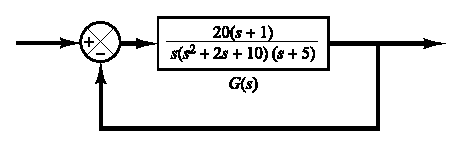
\includegraphics[width=8cm]{exercise1.eps}
	\end{figure}

	\item Considere un sistema de control con retroalimentación unitaria con la siguiente función de transferencia de lazo abierto:
	\begin{equation*}
		G(s) = \frac{K}{s(s^2+s+4)}
	\end{equation*}
	Determine el valor de la ganancia $K$ tal que el margen de fase sea \ang{50}. Cuál es el margen de ganancia para esta ganancia $K$?

	\item Considere el sistema mostrado en la figura. Dibuje el diagrama de Bode de la función de transferencia de lazo abierto y determine el valor de la ganancia K tal que el margen de fase sea \ang{50}. Cuál es el margen de ganancia del sistema con esta ganancia $K$?
	\begin{figure}[h]
		\centering
		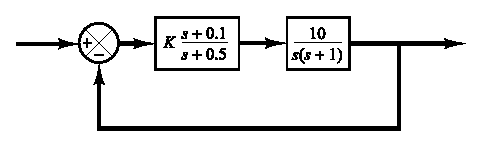
\includegraphics[width=10cm]{exercise3.eps}
	\end{figure}

	\item Considere el sistema de la figura. Se desea diseñar un compensador de adelanto $G_c(s)$ tal que el margen de fase sea $\ang{45}$, el márgen de fase no sea menor de 8 dB, y la constante de error de velocidad estática $K_v = 40$. Grafique las respuestas ante paso y rampa unitarias del sistema compensado.
	\begin{figure}[h]
		\centering
		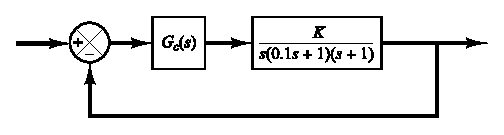
\includegraphics[width=10cm]{exercise4.eps}
	\end{figure}
 
\end{enumerate}

\end{document}